\documentclass[conference]{IEEEtran}
\usepackage{graphicx}
\usepackage{cite}
\usepackage{url}
\usepackage[cmex10]{amsmath}
\usepackage{algorithmic}
\usepackage{array}
\usepackage{mdwmath}
\usepackage{mdwtab}
\usepackage{eqparbox}
\usepackage[font=footnotesize]{subfig}
\usepackage{fixltx2e}

\begin{document}

\title{\large{CS388 NLP Project Proposal}\\ \huge{Text-based Mining for Hidden Relations and Trending}}

\author{\IEEEauthorblockN{C. Vic Hu}
\IEEEauthorblockA{vic@cvhu.org}
\and
\IEEEauthorblockN{Ali Unwala}
\IEEEauthorblockA{aliunwala@gmail.com}
}
\maketitle

\section{Motivation}
In economics and statistics, knowledge spillovers between researchers and inventors in close regions and similar domains have been studied to show strong influence \cite{Spillover1} \cite{Spillover2}. In this paper, we want to focus on implicit relations between US patents based on their terminology usage and writing styles. Furthermore, we will utilize the obtained knowledge relations to formalize hidden topics and make trend prediction.

\section{Objective}

Our main objectives are two folds. Firstly, we will build language models enhanced from ones proposed in \cite{Authorship} for each authors, years and patent classification numbers. Secondly, we wish to observe some hidden patterns correlated to years and classification numbers obtained from our first results, and construct a Markov Model to predict invention sequence and trending.

\section{Data Source}
Most of the text-based patents can be found on the US Patent and Trademark Office website \cite{uspto}. Although their out-dated markups and ambiguous formatting make it challenging to obtain clean and consistent data, we have spent some time on writing a simple web crawler and scraped around 700 documents. Each document has the following attributes of interest: 
\begin{enumerate}
\item Patent number
\item Authors (with location)
\item Classification numbers
\item Abstract
\item Claims
\item Description
\end{enumerate}

\section{Hypothesis}
Based on the authorship prediction model presented in \cite{Authorship}, we assume that similar patterns could be formulated in the context of US patents. In addition, we assume hidden topics exist and can be discovered over some patterns, and that their causal relationships can be established in a chronological order. 

\section{Method}
To build language models for capturing authorship, chronological and topic patterns, we will adapt and enhance the existing Penn-treebank-based probabilistic context-free grammar and maybe some bag-of-word methods such as topic modeling. To establish hidden sequence models \cite{HMM} and their relations with the observables (patent data), we will use some variations of the forward-backward algorithm to estimate relevant conditional probabilities and state transitions. 

\begin{figure} 
  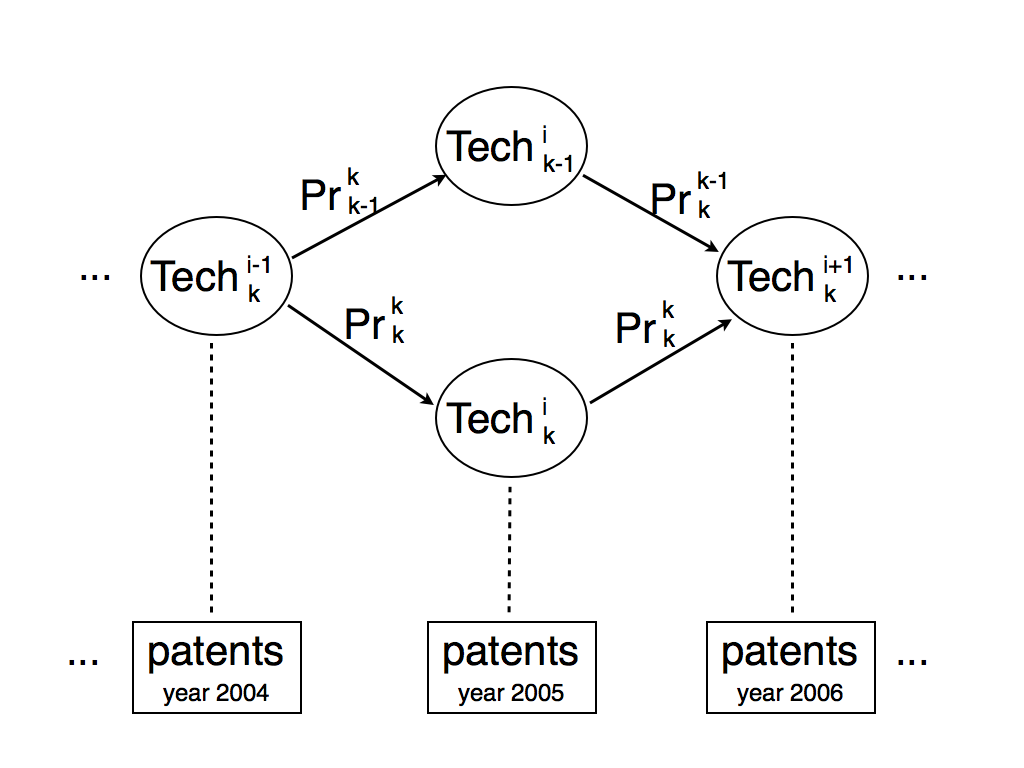
\includegraphics[width=0.5\textwidth]{hmm.png}
   \caption{Patents can be treated as observables for a hidden sequence of technology topics HMM}
\end{figure}

\section{Evaluation}
To evaluate our work, we wish to focus on patents in solar and wind energy from 2003 to 2012. For the first part of attribute predictions (authorships, years and classification numbers), we can simply hold out a subset as our testing data and compare our predictions accordingly. For the second part of hidden relation discovery, we can train older patent data on our algorithm, and compare our generated predictions with the newer patent data.


\begin{thebibliography}{1}

%\bibitem{IEEEhowto:kopka}
%H.~Kopka and P.~W. Daly, \emph{A Guide to \LaTeX}, 3rd~ed.\hskip 1em plus  0.5em minus 0.4em\relax Harlow, England: Addison-Wesley, 1999.

\bibitem{uspto}
http://uspto.gov

\bibitem{HMM}
D.~Ramage, \emph{Hidden Markov Models Fundamentals}, CS299~Section~Notes, 2007.

\bibitem{Authorship}
S.~Raghavan, A.~Kovashka and R.~Mooney, \emph{Authorship Attribution Using Probabilistic Context-Free Grammars}, Proceedings of the 48th Annual Meeting of the Association for Computational Linguistics, 38-42, 2010.

\bibitem{Spillover1}
F.~G.~Braun, J.~Schmidt-Ehmcke and P.~Zloczysti, \emph{Innovative Activity in Wind and Solar Technologies: Empirical Evidence on Knowledge Spillovers Using Patent Data}, CEPR Discussion Paper 7865, 2010.

\bibitem{Spillover2}
S.~Breschi and F.~Lissoni, \emph{Knowledge Spillovers and Local Innovation Systems: A Critical Survey}, Industrial and Corporate Change, Volume 10 Number 4, 2001.

\end{thebibliography}




% that's all folks
\end{document}


